\icode{E-MK-CA-L2-260928-002}
如图所示，子弹的初速度大小 \(v_{10} =\) \qty{150}{m/s}，足球的初速度大小 \(v_{20} =\) \qty{15}{m/s}，方向均水平向右。设它们与木板作用的时间均为 \(t = \) \qty{0.05}{s}。
\begin{enumerate}
	\item 若子弹击穿木板后瞬间的速度大小变为 \(v_1 =\) \qty{50}{m/s}、方向不变，求子弹击穿木板过程中的平均加速度大小 \(a_1\) 及方向;
	\item 若足球与木板作用后反向弹回的速度大小 \(v_2 =\) \qty{7}{m/s}，求足球与木板碰撞反弹过程中的平均加速度大小 \(a_2\) 及方向。
\end{enumerate}

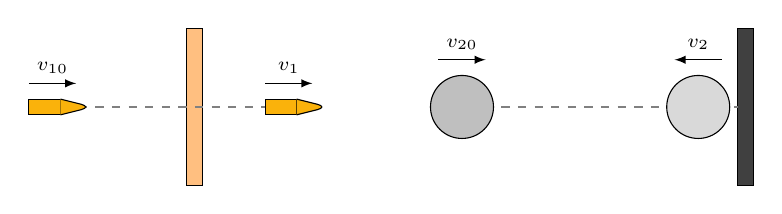
\begin{tikzpicture}[font=\scriptsize,>=latex]
	\begin{scope}
		\draw[fill=orange!50] (2,1) rectangle(2.2,-1);
		\draw[gray,dashed] (0,0)--(3,0);
		\draw[fill=yellow!70!red] (0,.1) rectangle(.4,-.1);
		\draw[rounded corners,fill=yellow!70!red] (.4,.1)--(.8,0)--(.4,-.1);
		\draw[fill=yellow!70!red] (3,.1) rectangle(3.4,-.1);
		\draw[rounded corners,fill=yellow!70!red](3.4,.1)--(3.8,0)--(3.4,-.1);
		\draw[->] (0,.3)--node[above]{\(v_{10}\)}(.6,.3);
		\draw[->] (3,.3)--node[above]{\(v_1\)}(3.6,.3);
	\end{scope}
	\begin{scope}[xshift=6cm]
		\draw[fill=gray!50!black] (3,1) rectangle(3.2,-1);
		\draw[gray,dashed] (0,0)--(3,0);
		\draw[fill=gray!50] (-.5,0) circle(.4);
		\draw[fill=gray!30] (2.5,0) circle(.4);
		\draw[->] (-.8,.6)--node[above]{\(v_{20}\)}(-.2,.6);
		\draw[->] (2.8,.6)--node[above]{\(v_2\)}(2.2,.6);
	\end{scope}
\end{tikzpicture}
\begin{answer}
	（1）\(a_1 = \) \qty{2000}{m/s^2}，水平向左（2）\(a_2 =\) \qty{440}{m/s^2}，水平向左
\end{answer}